\chapter{Motion and Forces}

\section{Describing Motion}

\begin{tcolorbox}[colback=red!5!white,colframe=red!75!black]
  \[\text{Average Speed}=\frac{\text{Distance}}{\text{Time}}\]
\end{tcolorbox}

If an object’s speed is changing throughout the distance measured, like a car speeding up as it gets on the highway, then this equation gives us its average speed during that time.

\vspace{.3cm}

\begin{figure}[htb!]
  \centering
  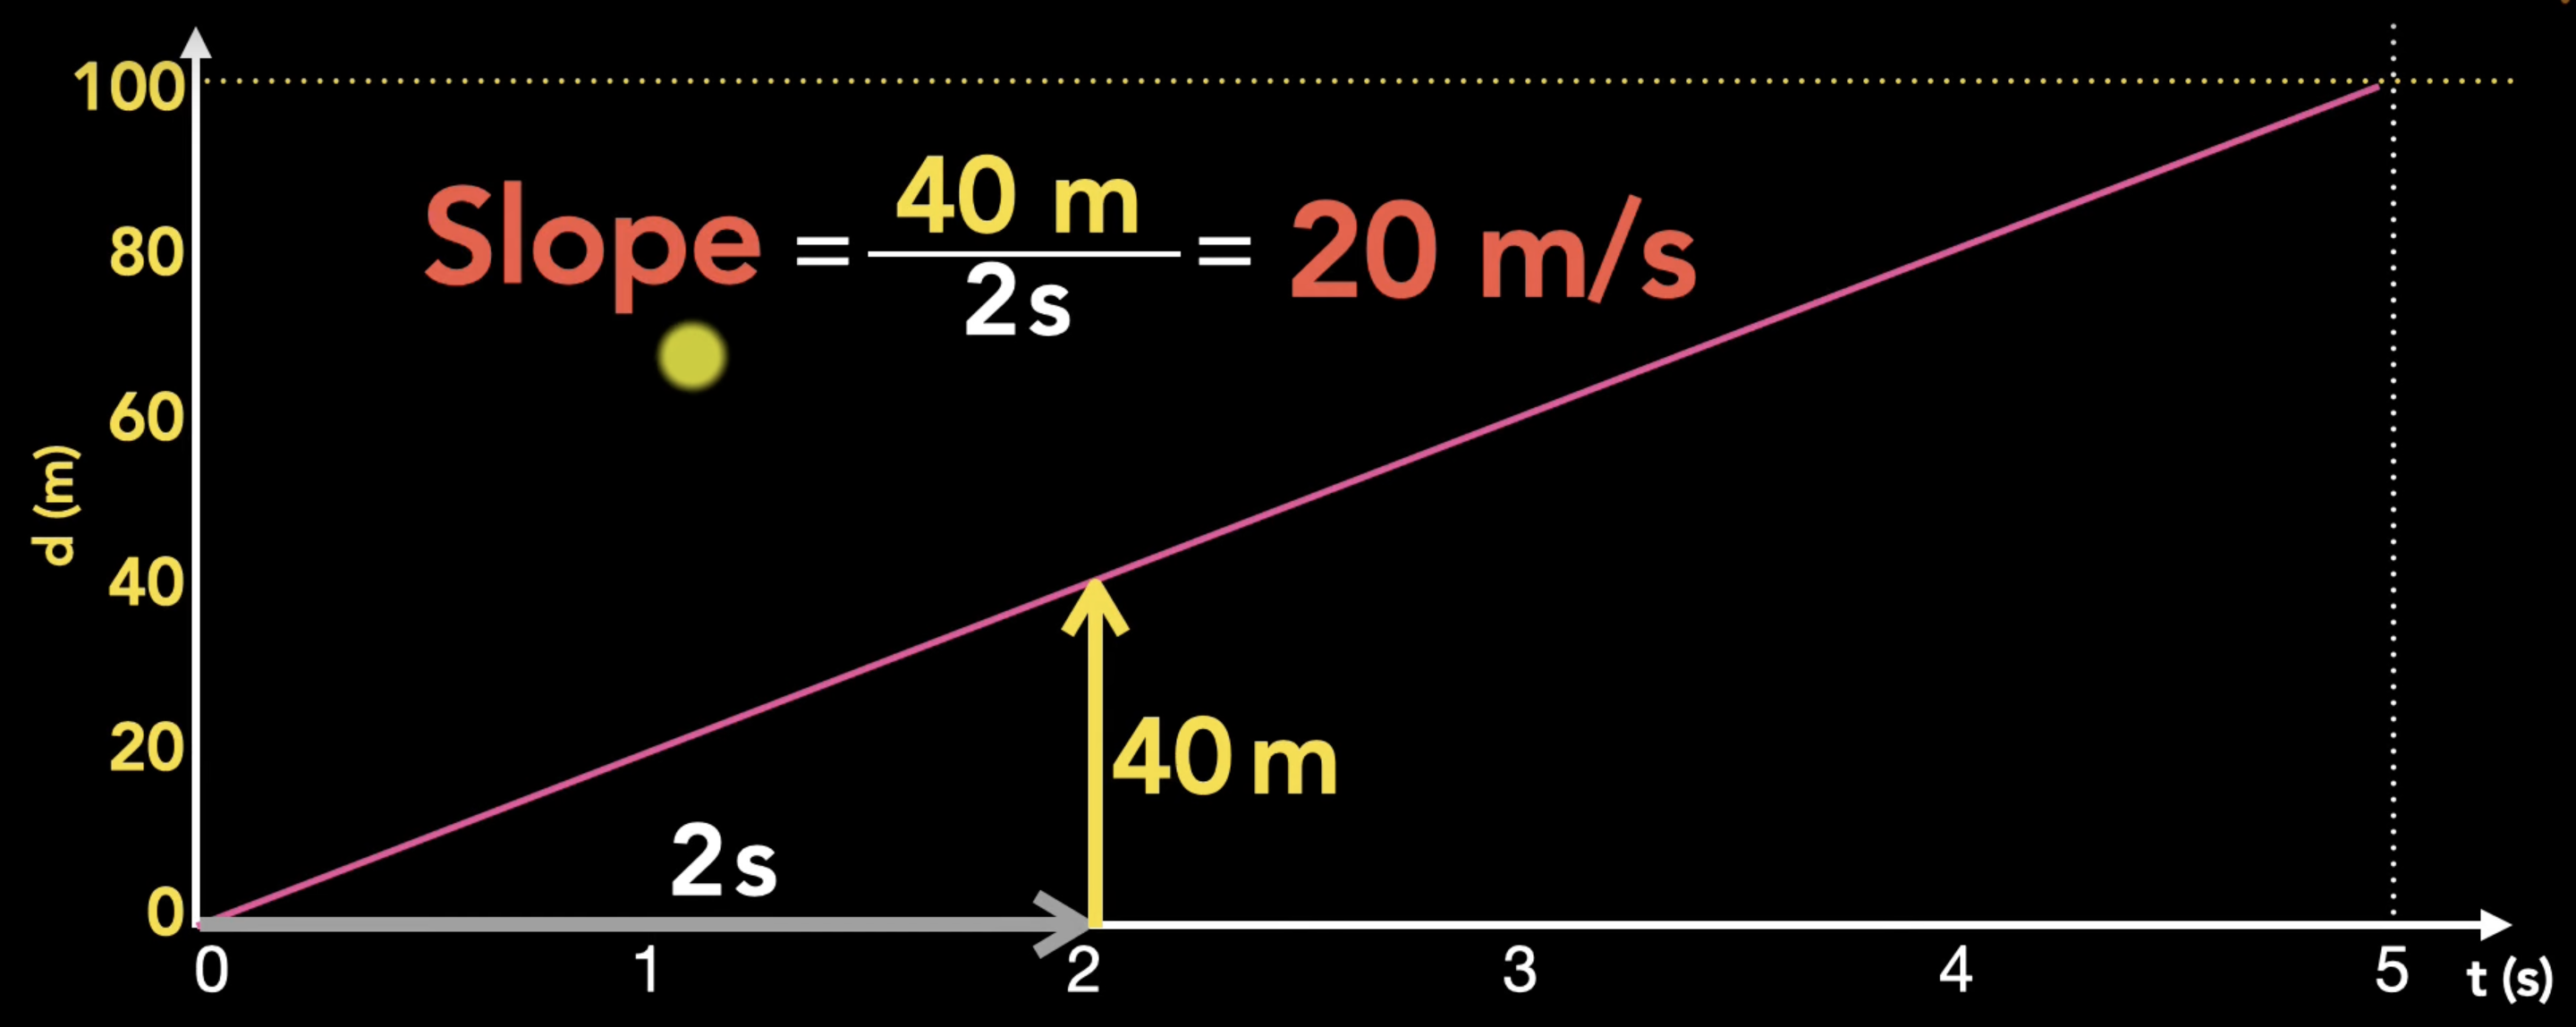
\includegraphics[width=0.8\textwidth]{0101.png}
  \caption{Graph of Speed}
\end{figure}

A \textbf{distance-time graph} shows the amount of time an object travels on the a-axis and the distance it travels in that time on the y-axis. The Speed of the object equals the \textbf{Slope} of the line.

\vspace{.5cm}

\hl{Velocity} (vận tốc) is speed plus direction. It measures how fast and in what direction an object moves.

% \vspace{.5cm}
\noindent\rule{\textwidth}{0.4pt}

\hl{Acceleration} measure how quickly the velocity of an object changes. Like velocity, it also has direction. Whenever an object is speeding up or slowing down, whenever its velocity changes, we say that object is accelerating.

If an object is speeding up, its velocity and acceleration are in the same direction. If an object is slowing down, its velocity and acceleration are in opposite directions.

An object is accelerating if its speed, direction, or both are changing. If neither an object's speed or direction are changing, it's moving at constant velocity and its acceleration is zero.

A car moving in a circle has constant velocity but changing direction, therefore it has acceleration.

\noindent\rule{\textwidth}{0.4pt}

Motion is a relative concept. It is relative to \textbf{reference frames}. There is no absolute motion or real motion.

From the sun or the moon's perspective (reference frame), the ground is moving.

Whether an object is at rest or in motion depends on the choice of reference frame. No one reference frame is more valid than another.

\noindent\rule{\textwidth}{0.4pt}

\hl{Distance} measures the length of the path travelled between two points. It doesn't include direction.

\hl{Position} measures the length and direction of a straight line from a reference point to an object's location. It is a vector. Example: 4 meters to the left.

If an object begins at the reference point and travels in a straight line, then its position and distance travelled are the same amount. But if it starts away from the reference point or turns along the way, then they're different.

\hl{Displacement} only concerns about the start point and the end point. It does not care how the object move from start to end.

\section{Forces}

A \hl{force} is a push or a pull. Its unit is Newtons - N.

Types of \textbf{contact forces} include the normal and friction forces. Types of \textbf{non-contact forces} include the gravitational, electric, and magnetic forces.

A \textbf{Normal Force} pair is produced when two surfaces press against each other. Each normal force acts perpendicular to the surface it’s applied to. (In math, \textit{normal} means perpendicular.)

\textbf{Friction} is a force that resists the relative motion of two surfaces in contact. It is parallel to the surface.

\vspace{.5cm}

When two or more forces act on an object in the same direction, their effects add. In opposite directions, their effects subtract. Adding and subtracting all of the individual forces this way gives the \hl{net force} on the object.

If the net force is zero, the forces are balanced. If not zero, the forces are unbalanced.

\noindent\rule{\textwidth}{0.4pt}

All forces are produced by two objects \textbf{interacting}. An object can’t change its motion by pushing or pulling on itself. \hl{Newton's third law} states that two interacting objects exert \underline{equal and opposite} forces on each other.

Each object in the pair experiences one of the forces in the pair. The forces in the pair have equal strengths even if the two interacting objects have different masses or speeds.

The forces in the pair don't balance (or cancel) each other out because they act on two different objects. When determining the net force on an object, we only consider forces that act \underline{on that object}. So, even though every force is part of a pair, we only model the one force from the pair that acts on the object we're analyzing.

When we say that two forces are \textbf{balanced}, it means that the forces must act on \underline{the same} object, point in opposite direction, and have the same strength.

For example, when a skater’s foot pushes backward against the ground, the ground pushes forward on the skater’s foot. This makes the skater accelerate forward.

\vspace{.5cm}

Newton's third law helps us understand how objects exert forces on \textbf{each other}. Newton's first and second laws will tell us how the forces exerted on an object affect its motion. 

\section{Connecting motion and forces}

\hl{Newton's First Law}: If the forces acting on object are balanced (the \textcolor{cyan}{net force} is \textcolor{cyan}{zero}), the object will not accelerate. It will remain at rest \textbf{OR} keep moving with constant velocity. If the forces acting on object are unbalanced (the net force is not zero), the object will accelerate. Its speed and/or direction of motion will change.

The statements also work in reverse. If we observe an object’s velocity changing, we can infer that the forces acting on it are unbalanced. If its velocity stays constant, we know the forces acting on it are balanced:

Remember that velocity includes both speed and direction. So if an object is not moving in a straight line, its velocity is changing. Therefore, the forces acting on a turning object are unbalanced.

An unbalanced force can cause an object to speed up, slow down, and/or change direction. The result depends on the direction the unbalanced force acts compared with the direction the object is moving:

\begin{itemize}
  \item If the net force acts in the same direction the object is moving, the object speeds up.
  \item If the net force acts opposite the direction the object is moving, the object slows down.
  \item If the net force acts at an angle compared to the direction the object is moving, the object changes direction.
\end{itemize}

\vspace{.4cm}

\hl{Newton's Second Law}: If the forces on an object are unbalanced (the net force is NOT zero), the object will accelerate. How much the object accelerates depends on two factors: the strength of the net force, and the mass of the object.

\begin{itemize}
  \item If we keep the object's mass constant and increase the net force, we find that the object accelerates more.
  \item If we keep the net force constant and increase the object's mass, we find that the object accelerates less.
\end{itemize}

We can express Newton’s second law as an equation:

\begin{tcolorbox}[colback=red!5!white,colframe=red!75!black]
  \[\text{acceleration}=\frac{\text{net force}}{\text{mass}}\]
\end{tcolorbox}

Newton's laws accurately describe situations we encounter in our everyday lives. However, to analyze the motion of very small objects (the size of atoms or smaller) we need quantum mechanics. And for objects moving near the speed of light we need Einstein's theory of special relativity.
